\chapter{Design and Implementation}
\label{chap:design}
This chapter will present the design and technical details on the implementation of Sociopath event extraction system. In the \nameref{sec:method} we will discuss our method and set the problem formulation, also we will briefly walk through the main points of the project's workflow. We will recapitulate the information on Microdata from the chapter \nameref{chap:background}and explain how it is relevant in the context of event extraction process. The main part of this section is devoted to the process of training dataset construction. \\

In the section \nameref{sec:arch} we will show the diagram of the project and describe the basic components. 

\section{Methodology and Approach}
\label{sec:method}
As we mentioned in \nameref{chap:intro}, the Sociopath system aims to extract the following four event properties from the web page: 

\begin{enumerate}
    \item The title
    \item The description
    \item The date and time
    \item The certain location where event is taking place
\end{enumerate}

As also said we assume that the page already contains an event announcement, and we don't solve the task of information retrieval to list those pages which contain the events. Our task is to find and extract the structured information about the event knowing it's actually there.\\

We consider the event extraction problem as several binary classification tasks, where every model runs on every element of the web page and makes its decision. In our approach, we explicitly build one-vs-all classifiers for every event component. Thus we have 4 different models that independently process the elements of the web page. \\

On the web page, there are a big number of elements which are not relevant by default and even can't be considered as an event property. The list of such elements includes advertisement blocks and pop-ups, footers, sidebars, media and other elements which are expected to be on a regular web page. We don't want our classifiers to spend computational time on such elements so we applied the filtering procedure in order to leave only relevant web elements for further analysis.\\

\subsection{About the dataset}
As usual, for building the meaningful statistical model one need to have a relatively large training set. As it was said before the collecting of such dataset is one of the main problems in Informational Extraction and often implies human involvement into labeling procedure. In our case we must have a big set of web pages with event announcement for which we know exactly where every component is located. One of the 'location' identifiers of the web element is XPath of the element in a DOM tree. What is XPath we discussed in details in the chapter \nameref{chap:background}.\\

There are various types of design and structure of an event page. The event components might be located in different places relative to each other. Furthermore, there are different HTML code styles, which depends on the developer who programmed the front-end, used web frameworks and technologies. In order to build the model which will work on previously unseen web pages, we must train the classifiers on many diverse pages to consider all these cases. That's the reason why didn't consider the option of collecting the training dataset through the human labeling process.\\   

As we will discuss in the chapter \nameref{chap:datacollect} there are exist several non-free well-formed datasets for 'vertical services' tasks. Researchers in related projects have been used these datasets and showed the high performance. In this thesis we didn't consider paid datasets as an option and rather set as a goal to create a technique for collecting such dataset automatically.\\

To generate the dataset for training and evaluation we exploited the set of web pages which format their HTML code using the semantic markup Microdata together with the schema \textit{Event} from Schema.org. The Microdata markup and its structure were previously discussed in details in \nameref{chap:background} chapter. Search engines take advantage of the semantic markup to automatically extract the information, incorporate it into its vertical services and provide a richer browsing experience for users. Despite the fact search engines encourage and promote the websites which use such markup, in fact, not all of them use it. By statistics only 16\% of the domains use semantic markup, the rest 84\% use classic HTML. That's also the reason why the task of structural information extraction from unstructured web pages is still relevant - most of the data on the Internet is still stored as a plain HTML.\\ 

Stat Link: http://webdatacommons.org/structureddata/2016-10/stats/stats.html  \\

In order to extract the information from the web pages which actually do use the semantic Microdata tags, first of all, we need to find these pages and select only those ones which contain an event announcement. As we said, there is only small part of such websites. That means the problem of gathering the pages with specific schema is not obvious especially if we want to collect the rich and diverse dataset of URLs. As a consequence, one of the intermediate tasks in the thesis was to collect the list of URLs which apply Microdata with Event schema in their HTML code. \\

Fortunately for us, we discovered the great open repository \textit{Common Crawl}, which maintains and collects the web crawl unstructured data. Common Crawl is the largest web corpus available to the public, which collects petabytes of data from various Internet pages. To find the pages which contain the Event Microdata markup would not be feasible if it wasn't for another great open repository \textit{Web Data Commons} which in fact does what we exactly need - it annually processes the Common Crawl entire database and selects only those URLs which contain any kind of structured data including RDFa, Microdata, Microformat, and Embedded JSON-LD. \\

The detailed process of collecting URLs, cleaning, parsing those URLs and again cleaning is discussed in the chapter \nameref{chap:datacollect}. The most challenging part of data collection task was the parsing those list of URLs. We had 80GB of URLs which supposed to contain an Event schema. We went through all of them, checked they availability, found the web elements tagged with Microdata semantic markup and extracted corresponding web features. For these purposes we implemented continuous parallel crawling process and set it on MetaCentrum computers. The result of all these steps is a dataset where every row consists of a URL, event component name and the values of corresponding features which we extracted from the page.\\ 

After we created the dataset we performed the following procedures:
\begin{enumerate}
    \item Comprehensive exploratory data analysis including visualization of extracted features for every event component.
    \item We performed feature engineering in order to extract useful information from text features, spatial features (X and Y coordinates of the web element) and visual features (CSS). 
    \item Since we will work with several hundreds features, we run dimensionality reduction and feature selection methods. 
    \item We built several models for binary classification tasks, optimized parameters for every model and presented comparison tables.  
    \item We evaluated the models on previously unseen data.    
\end{enumerate}

\section{Architecture of the system / TODO}
\label{sec:arch}

The system is composed of 4 logical modules:

\begin{itemize}
    \item \textbf{I. URLs Collection} - download data from Web Data Commons, clean it, extract the URLs with Event Microdata semantic markup.
    \item \textbf{II. Creating a dataset} - send these URLs to MetaCentrum and set continuous parallel crawling process for extracting web elements of the event components and corresponding features.
    \item \textbf{III. Dataset cleaning} - processing of the raw data, in the end we'll have a final dataset for analysis.
    \item \textbf{IV. Analysis and modeling} - data exploration, analysis, building and evaluation of models.
\end{itemize}

On the picture below you see the detailed schema of the application. 

\begin{figure}[h]
\begin{center}
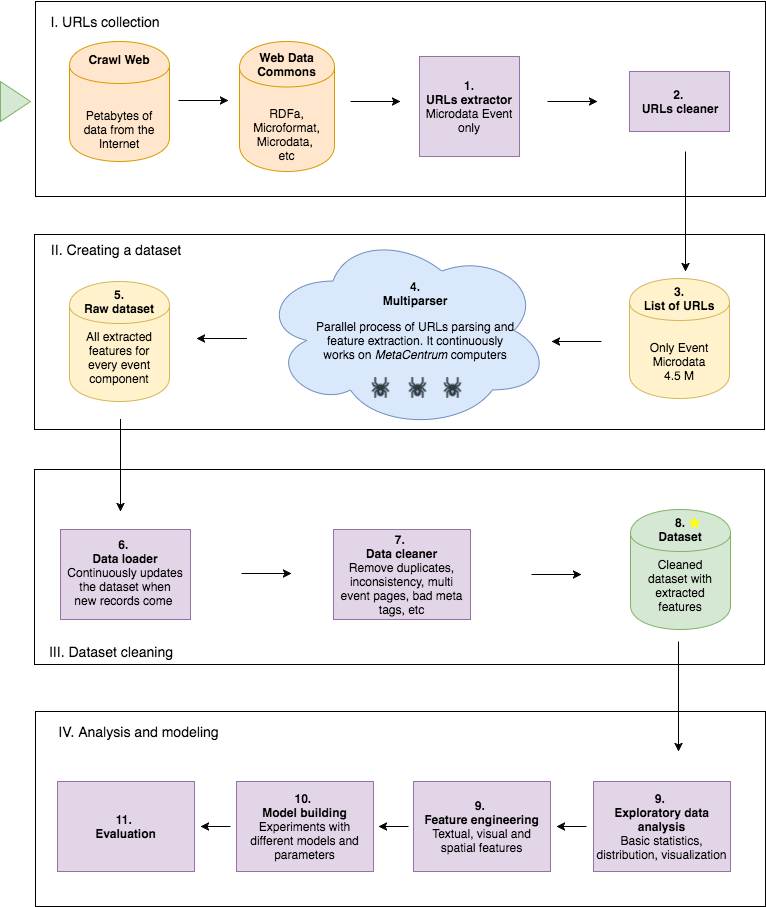
\includegraphics[width=1.0\textwidth]{figures03/Architecure}
\caption{The components of Sociopath event extraction system}
\label{fig:architecture}
\end{center}
\end{figure}

\vspace{5mm} 
\noindent\textbf{Common Crawl}\\\\
\textit{The Common Crawl Foundation} is non-profit organization which collects and maintain the largest and the most comprehensive public corpus of web crawl data. Common Crawl's web archive consists of more than 250 TiB of content from more than 3 billion webpages. It completes the crawls every month and the history is available for the last 8 years (http://commoncrawl.org/connect/blog/). Common Crawl keeps the data in AWS S3 bucket which publicly available by this link https://aws.amazon.com/ru/public-datasets/common-crawl/  The corpus contains raw web page data, extracted metadata (RDFa, Microdata, Microformat, etc) and extracted text. \\

\vspace{5mm} 
\noindent\textbf{Web Data Common}\\\\
% AMAZON article, edit
\textit{The Web Data Commons} (WDC) project was started by researchers from Freie Universität Berlin and the Karlsruhe Institute of Technology (KIT) in 2012. The goal of the project is extracting the structured data (RDFa, Microdata, Microformat, and Embedded JSON-LD) from the Common Crawl corpus and share the dataset for public download in order to support researcher and companies.The same as Common Crawl corpus, structured corpus is publicly available in Amazon S3 buckets.

\vspace{5mm} 
\noindent\textbf{1. URLs extractor}\\\\
\vspace{5mm} 
\noindent\textbf{2. URLs cleaner}\\\\
\vspace{5mm} 
\noindent\textbf{3. List of URLs}\\\\
\vspace{5mm} 
\noindent\textbf{4. Multiparser}\\\\
\vspace{5mm} 
\noindent\textbf{5. Raw dataset}\\\\
\vspace{5mm} 
\noindent\textbf{6. Data loader}\\\\
\vspace{5mm} 
\noindent\textbf{7. Data cleaner}\\\\
\vspace{5mm} 
\noindent\textbf{8. Dataset}\\\\
\vspace{5mm} 
\noindent\textbf{9. Exploratory data analysis}\\\\
\vspace{5mm} 
\noindent\textbf{10. Feature engeneering}\\\\
\vspace{5mm} 
\noindent\textbf{11. Model building}\\\\
\vspace{5mm} 
\noindent\textbf{12. Evaluation}\\\\

\section{Tools / TODO}


